\chapter{Conception Préliminaire}
%\addcontentsline{toc}{chapter}{Conception Préliminaire}
\thispagestyle{fancy}
\lhead{Conception Préliminaire}

\section{Diagramme du cas d'utilisation}

Ci-dessous se trouve le diagramme présentant le cas d'utilisation présentant le déroulement d'une partie:
    
\begin{figure}[h!]
\begin{center}
\includegraphics[width=.8\linewidth]{../conception/CasDUtilisation.pdf}
\caption{Cas d'Utilisation du déroulement d'une partie}
\end{center}
\end{figure}


\newpage
\section{Diagramme de séquence système}
Ci-dessous se trouve le diagramme de séquence système illustrant le cas d'utilisation présenté précédemment:
\begin{figure}[h!]
\begin{center}
\includegraphics[width=.8\linewidth]{../conception/DSS.pdf}
\caption{DSS du déroulement d'une partie}
\end{center}
\end{figure}

\newpage
\section{Maquettes}
Notre interface web permet de visualiser une partie en cours. Elle n'est constituée que d'une unique page. Voici une maquette de cette page:

\begin{figure}[h!]
\begin{center}
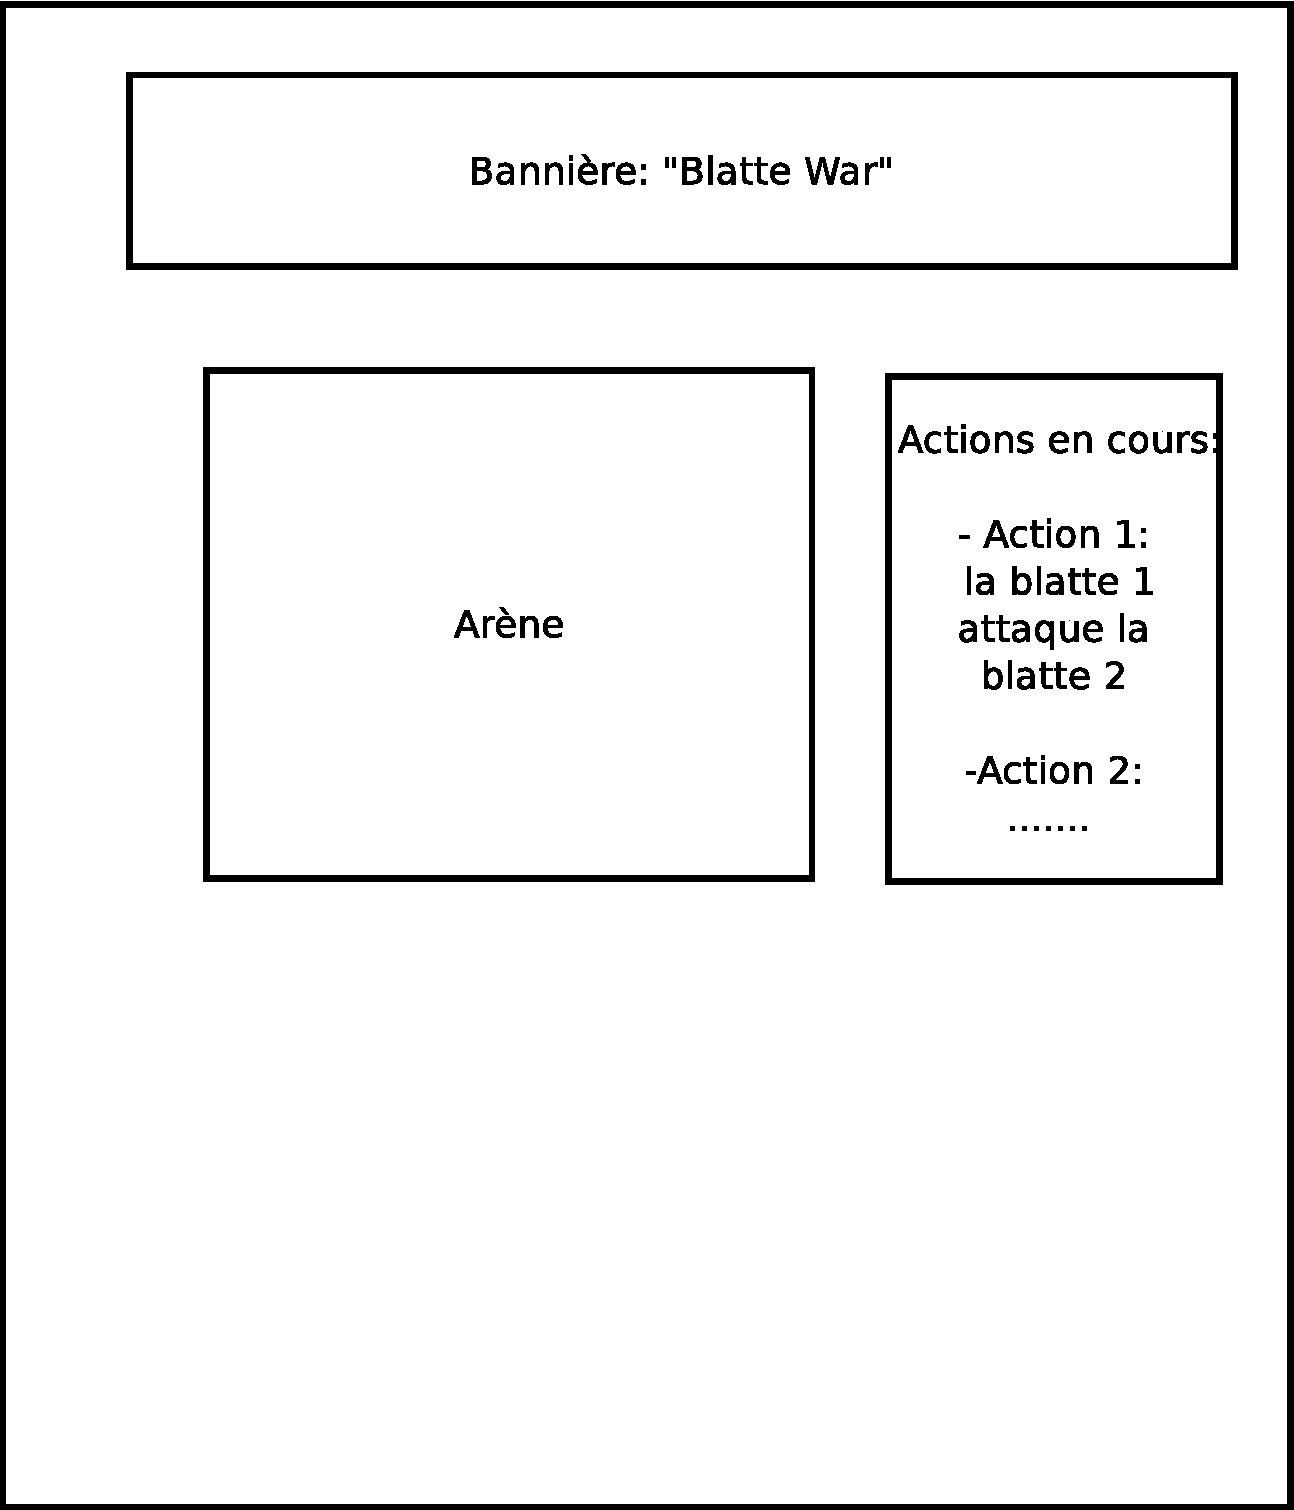
\includegraphics[width=.8\linewidth]{images/mockup.pdf}
\caption{Maquette de la page web (affichage de l'arène d'une partie en cours)}
\end{center}
\end{figure}


    
\newpage
\section{Diagramme de classe}
    L'implémentation du jeu devra respecter le diagramme de classe suivant :

    \begin{figure}[ht]
    \begin{center}
    \includegraphics[scale=0.32]{../conception/UML_Blatte.pdf}
    \end{center}
    \caption{Diagramme de classes, partie 1}
    \end{figure}

    \begin{figure}[ht]
    \begin{center}
    \includegraphics[scale=0.32]{../conception/UML_Blatte_p2.pdf}
    \end{center}
    \caption{Diagramme de classes, partie 2}
    \end{figure}

